\documentclass[12pt, a4paper]{article}

\usepackage[czech]{babel}
\usepackage{lmodern}
\usepackage[utf8]{inputenc}
\usepackage[T1]{fontenc}
\usepackage{graphicx}
\usepackage{amsmath}
\usepackage[hidelinks,unicode]{hyperref}
\usepackage{float}
\usepackage{listings}
\usepackage{tikz}
\usepackage{xcolor}
\usepackage[final]{pdfpages}
\usepackage{tabularx}

\definecolor{mauve}{rgb}{0.58,0,0.82}
\usetikzlibrary{shapes,positioning,matrix,arrows}

\newcommand{\img}[1]{(viz obr. \ref{#1})}

\definecolor{pblue}{rgb}{0.13,0.13,1}
\definecolor{pgreen}{rgb}{0,0.5,0}
\definecolor{pred}{rgb}{0.9,0,0}
\definecolor{pgrey}{rgb}{0.46,0.45,0.48}

\usepackage{url}

\usepackage[normalem]{ulem}
\hypersetup{colorlinks,urlcolor=blue}

% hack into hyperref
\makeatletter
\DeclareUrlCommand\ULurl@@{%
  \def\UrlFont{\ttfamily\color{blue}}%
  \def\UrlLeft{\uline\bgroup}%
  \def\UrlRight{\egroup}}
\def\ULurl@#1{\hyper@linkurl{\ULurl@@{#1}}{#1}}
\DeclareRobustCommand*\ULurl{\hyper@normalise\ULurl@}
\makeatother

\lstset{frame=tb,
  language=C,
  aboveskip=3mm,
  belowskip=3mm,
  showstringspaces=false,
  columns=flexible,
  basicstyle={\small\ttfamily},
  numbers=none,
  numberstyle=\tiny\color{gray},
  keywordstyle=\color{blue},
  commentstyle=\color{dkgreen},
  stringstyle=\color{mauve},
  breaklines=true,
  breakatwhitespace=true,
  tabsize=3
}

\lstset{language=Java,
  showspaces=false,
  showtabs=false,
  breaklines=true,
  showstringspaces=false,
  breakatwhitespace=true,
  commentstyle=\color{pgreen},
  keywordstyle=\color{pblue},
  stringstyle=\color{pred},
  basicstyle=\ttfamily,
  moredelim=[il][\textcolor{pgrey}]{$$},
  moredelim=[is][\textcolor{pgrey}]{\%\%}{\%\%}
}

\let\oldsection\section
\renewcommand\section{\clearpage\oldsection}

\begin{document}
	% this has to be placed here, after document has been created
	% \counterwithout{lstlisting}{chapter}
	\renewcommand{\lstlistingname}{Ukázka kódu}
	\renewcommand{\lstlistlistingname}{Seznam ukázek kódu}
    \begin{titlepage}

       \centering

       \vspace*{\baselineskip}

       \begin{figure}[H]
          \centering
          
\includegraphics[width=7cm]{img/fav-logo.jpg}
       \end{figure}

       \vspace*{1\baselineskip}
       {\sc Semestrální práce z předmětu KIV/MBKZ}
       \vspace*{1\baselineskip}

       \vspace{0.75\baselineskip}

       {\LARGE\sc Multiplatformní aplikace zobrazující předpověď počasí\\}

       \vspace{4\baselineskip}
       
		\vspace{0.5\baselineskip}

       
       {\sc\Large Stanislav Král \\}

       \vspace{0.5\baselineskip}

       {A17B0260P}

       \vfill

       {\sc Západočeská univerzita v Plzni\\
       Fakulta aplikovaných věd}


    \end{titlepage}


    \tableofcontents
    \pagebreak


   \section{Analýza}

	\subsection{Vývoj multiplatformních aplikaci pomocí frameworku Flutter}
Flutter je open-source framework na jehož vývoji se podílí převážně firma Google. Cílem Flutteru je nabídnout vývojářům možnost vyvíjet výkonné aplikace, které působí nativně na všech platformách. Flutter umožňuje sdílet veškerý kód mezi všemi platformami. Toho je docíleno tak, že knihovna nepoužívá žádné nativní komponenty uživatelského rozhraní dané platformy. Okno aplikace totiž pouze slouží jako plátno a~všechny komponenty si Flutter vykresluje sám. K~vykreslování používá open-source knihovnu Skia, která je napsaná v~jazyce C++, čímž dosahuje plynulosti ve zobrazování uživatelského rozhraní. Pro psaní Flutter aplikací se používá programovací jazyk Dart.

Flutter respektuje rozdíly v~chování uživatelských rozhraní mezi mobilními operačními systémy čímž pomáhá aplikacím psaným v~tomto frameworku působit tak, jako kdyby byly nativní a~cílené právě pro danou platformu. Mezi hlavní rozdíly mezi platformami, jež tato knihovna implementuje na jednotlivých platformách zvlášt, patří například \textbf{scrollování}, ikony nebo typografie.

Při nasazení na Android platformu je C a~C++ kód enginu je kompilován pomocí Android NDK, zatímco Dart kód se s~využitím kompilace typu ahead-of-time kompiluje do nativních ARM a~x86 knihoven. Tyto knihovny jsou poté použity ve vygenerované nativní Android aplikaci, která slouží jako hostitel, a~z~celého projektu je následně vytvořen APK balík. Při vyvíjení Flutter aplikace je použit virtuální stroj, který umožňuje upravovat zdrojový kód aplikace bez nutnosti ji restartovat. Tato funkcionalita má největší význam při tvorbě uživatelského rozhraní, kdy se jednotlivé změny v~designu aplikace ihned projeví na zařízení. Podobně probíhá i~nasazení aplikace na iOS platformu, kdy kód enginu je překládán pomocí LLVM. Kompilace do nativních knihoven znamená, že narozdíl od ostatních frameworků pro tvorbu multiplatformních aplikací, jsou Flutter aplikace zcela nativní.

\begin{figure}[!ht]
\centering
{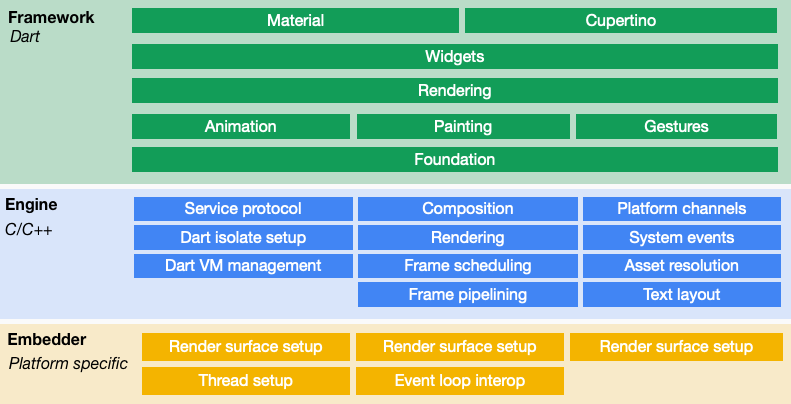
\includegraphics[width=13.5cm]{img/flutter-architecture.png}}
\caption{Diagram architektury Flutter}
\label{fig:flutter-architecture}
\end{figure}

Prvky uživatelského rozhraní, které Flutter nabízí, se snaží co nejvěrněji napodobit ty nativní. Prvky napodobující prvky platformy Android se nachází v~balíku \texttt{Material} a~prvky platformy iOS v~balíku \texttt{Cupertino}. Tým vývojářů Flutteru bere ohledy na aktualizace mobilních operačních systémů a~změny v~uživatelských rozhraní včasně implementuje do svého frameworku.

Flutter dále umožňuje psát nativní kód specifický pro danou platformu pomocí konstrukce zvané \texttt{platform channel}, která funguje na principu asynchronního předávání zpráv. Část Flutter aplikace pošle hostitelské nativní aplikaci zprávu, která asynchronně na tuto zprávu odpoví. Toto umožňuje přístup k~nativnímu API dané platformy.

Na konci roku 2019, v~každoročním shrnutí služby GitHub, je programovací jazyk Dart, který se v~dnešní době používá nejvíce právě ve Flutter aplikacích, označen jako jazyk s~nejrychleji rostoucím počtem vývojářů, jež ho používají pro vývoj aplikací.


\subsection{Výběr API pro získání dat předpovědi počasí}

Nutným předpokladem pro efektivní vývoj mobilní aplikace, která zobrazuje předpověď počasí, je správný výběr služby, jež zpřístupňuje API umožňující získávání dat obsahující předpověď počasí dle názvu města a tato data jsou v přehledně strukturovaná.


\subsubsection{Služba OpenWeather}

Služba OpenWeather \footnote{OpenWeather - \ULurl{https://openweathermap.org/api}} nabízí pro registrované uživatele tarifní plán zdarma, v rámci kterého lze přistupovat k API této služby, jež poskytuje dle názvu města data obsahující předpověď počasí pro danou oblast. Pro použití tohoto API je však nutné si nechat vygenerovat API klíč, který musí být použit při každém volání tohoto API. Data poskytována tímto API jsou dostupná ve formátu JSON, XML nebo HTML. Tato služba nabízí krátkodobou i dlouhodobou předpověď počasí a plán zdarma je omezen 1000 přístupy k API denně.


\subsubsection{Služba Weatherbit}

Tato služba, jež poskytuje v rámci svého zdarma tarifního plánu API poskytující předpověď počasí, umožňuje registrovaným uživatelům až 500 přístupů k předpovědím zdarma \footnote{Weatherbit - \ULurl{https://www.weatherbit.io/api}}. Toto API je pečlivě popsané a dokonce nabízí k dispozici dokumentaci pomocí služby \textbf{Swagger}.


\subsubsection{Služba MetaWeather}

Služba MetaWeather \footnote{MetaWeather - \ULurl{https://www.metaweather.com/}} slouží jako agregátor dat předpovědi počasí ze služeb \texbf{BBC}, \textbf{Forecast.io},  \textbf{HAMweather} nebo například \textbf{OpenWeather}, čímž slibuje větší přesnost svých předpovědí. API, které tyto agregované předpovědi poskytuje, je dostupné zdarma a bez jakýchkoliv omezení. Uživatel tohoto API je však povinen ve své práci uvést odkaz na webovou stránku této služby a neměl by toto API používat ke komerčním účelům. 

Poskytované API je velmi jednoduché a umožňuje vyhledávat konkrétní předpovědi pro dané lokace pomocí názvu měst. Nevýhodou této služby je to, že počet měst, pro které poskytuje předpověď počasí, je velmi malý. Například pro Českou republiku poskytuje předpověď pouze pro Prahu.


\section{Uživatelské rozhraní vytvořené aplikace}

Aplikace implementuje vlastní design uživatelského rozhraní, který je identický na obou hlavních mobilních platformách, a tak se přímo neřídí doporučeným designem iOS nebo Android aplikací.

\subsection{Úvodní obrazovka aplikace}

Na úvodní obrazovce aplikace je zobrazen název aplikace a logo frameworku Flutter. Pod těmito komponentami je umístěn seznam měst, ke kterým si uživatel již v minulosti vyhledal předpověd počasí. Pro tato města je automaticky získána aktuální předpověď počasí. Následně se pod tímto seznamem nachází vstupní pole, které slouží pro zadání názvu města, pro něhož si uživatel přeje zjistit předpověď počasí. Tlačítkem, jež je umístěno ve spodní části obrazovky, se spustí vyhledávání předpovědi počasí pro dané město.

\begin{figure}[h]
    \centering
    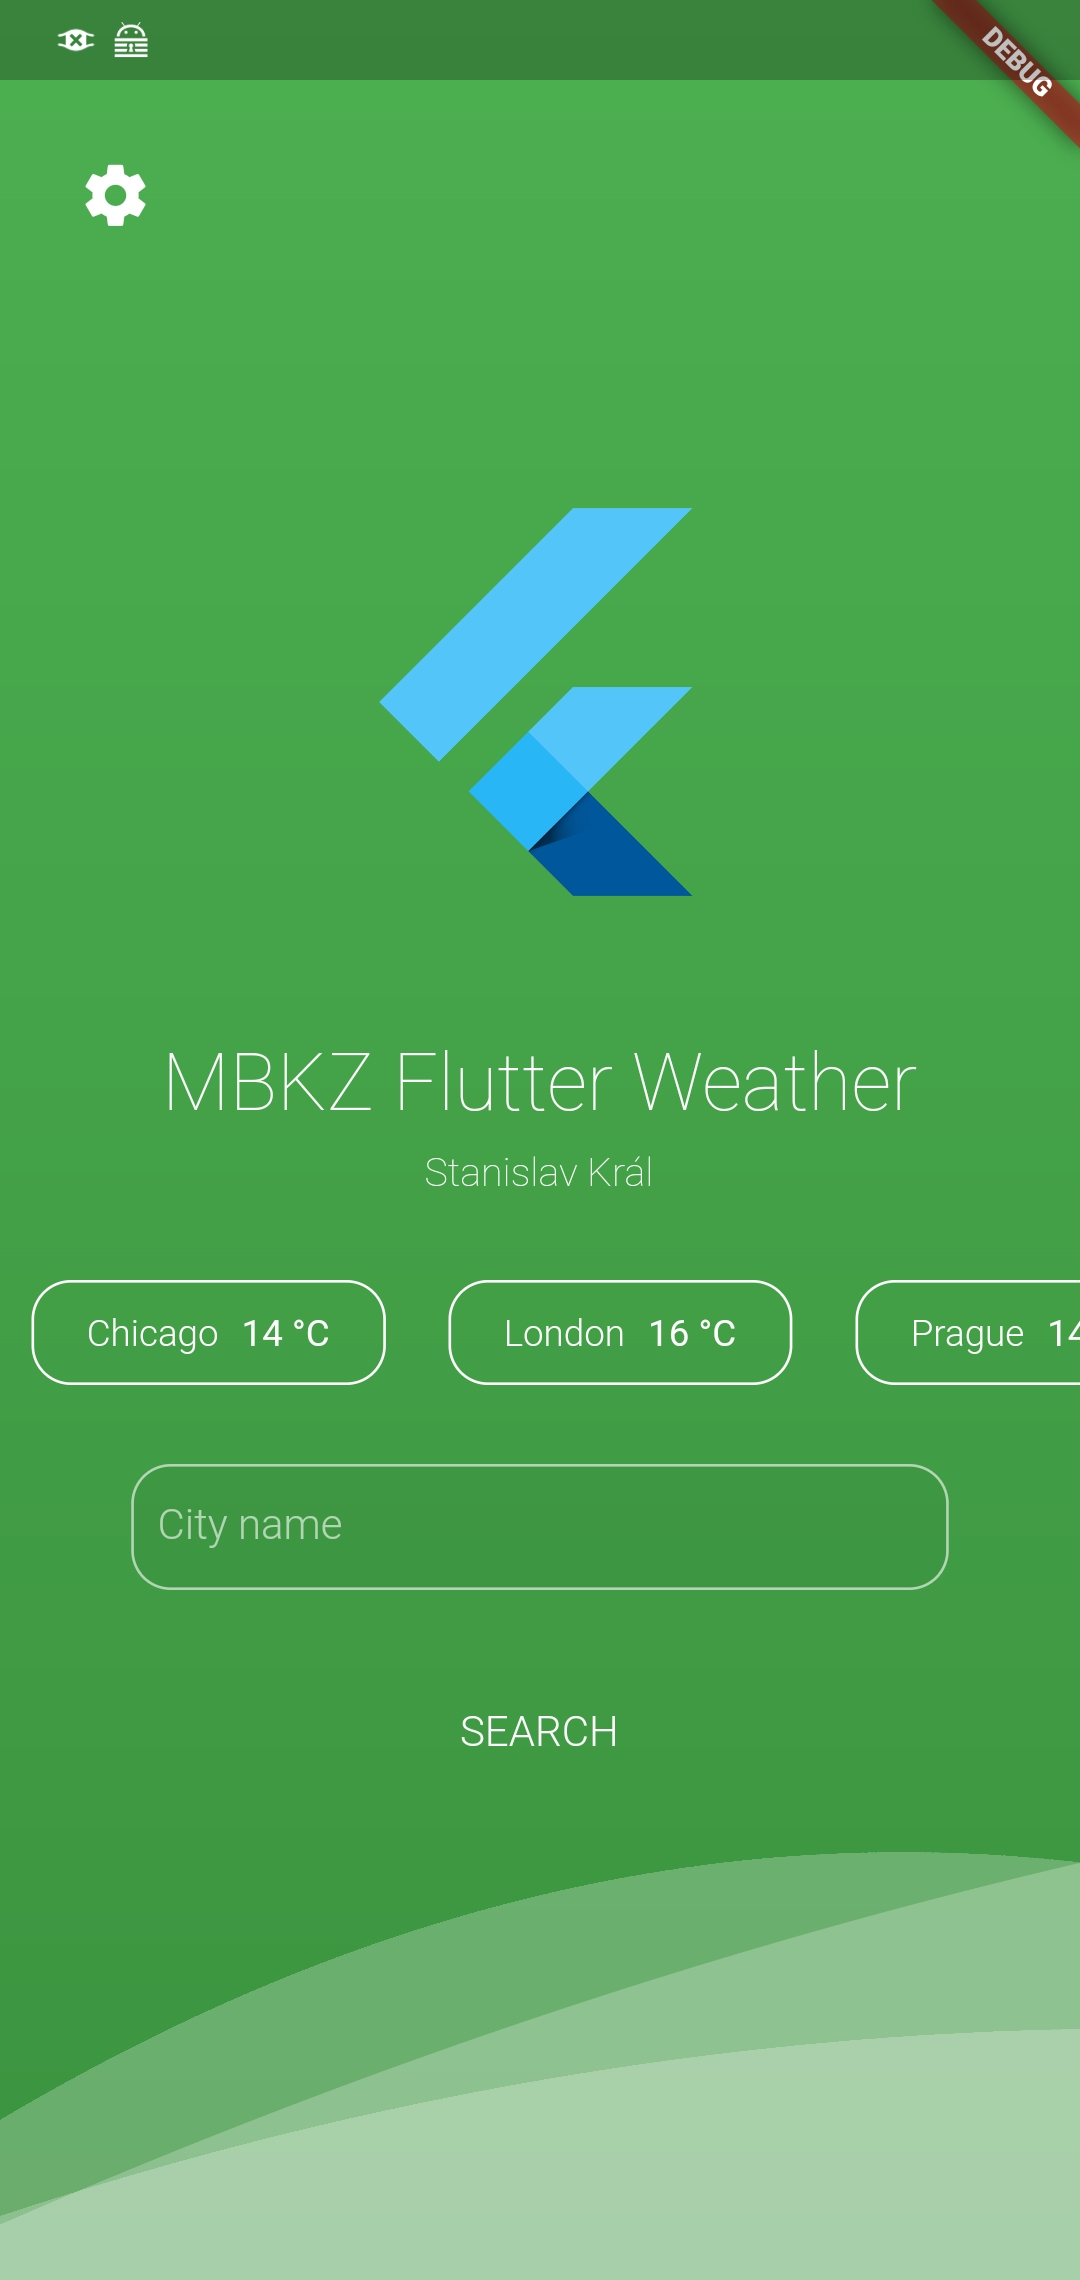
\includegraphics[width=0.40\textwidth]{img/app-menu.jpg}
    \caption{Úvodní obrazovka aplikace}
    \label{fig:mesh1}
\end{figure}

Pokud uživatel klikne na nějakou položku ze seznamu již vyhledaných měst, tak se otevře detailní předpověď pro vybrané město. Dlouhým stisknutím prstu na vybranou položku je tato položka z tohoto seznamu odebrána.

\subsection{Obrazovka předpovědi počasí}

Na této obrazce se nachází název města, ke kterému je aktuálně zobrazována předpověd počasí. Pod názvem města je zobrazené datum, ke kterému se předpověď vztahuje. Předpověď popisuje očekávané počasí za jeden konkrétní den. Uprostřed obrazovky je zobrazena předpovídaná průměrná teplota, minimální teplota a maximální teplota za daný den. Pod teplotami jsou zobrazeny informace o vlhkosti a rychlosti větru.

Horizontálním táhnutím prstu po obrazovce lze přepínat mezi předpověďmi na nadcházející dny (celkem 5 předpovědí). Každý hlavní typ počasí, které v daný den panuje, je reprezentován animovaným pozadím této obrazovky, jež se při změně typu mění a vizualizuje tak například když má v ten den pršet, sněžit nebo pokud má být jasná obloha.

\begin{figure}[!htb]
\minipage{0.32\textwidth}
  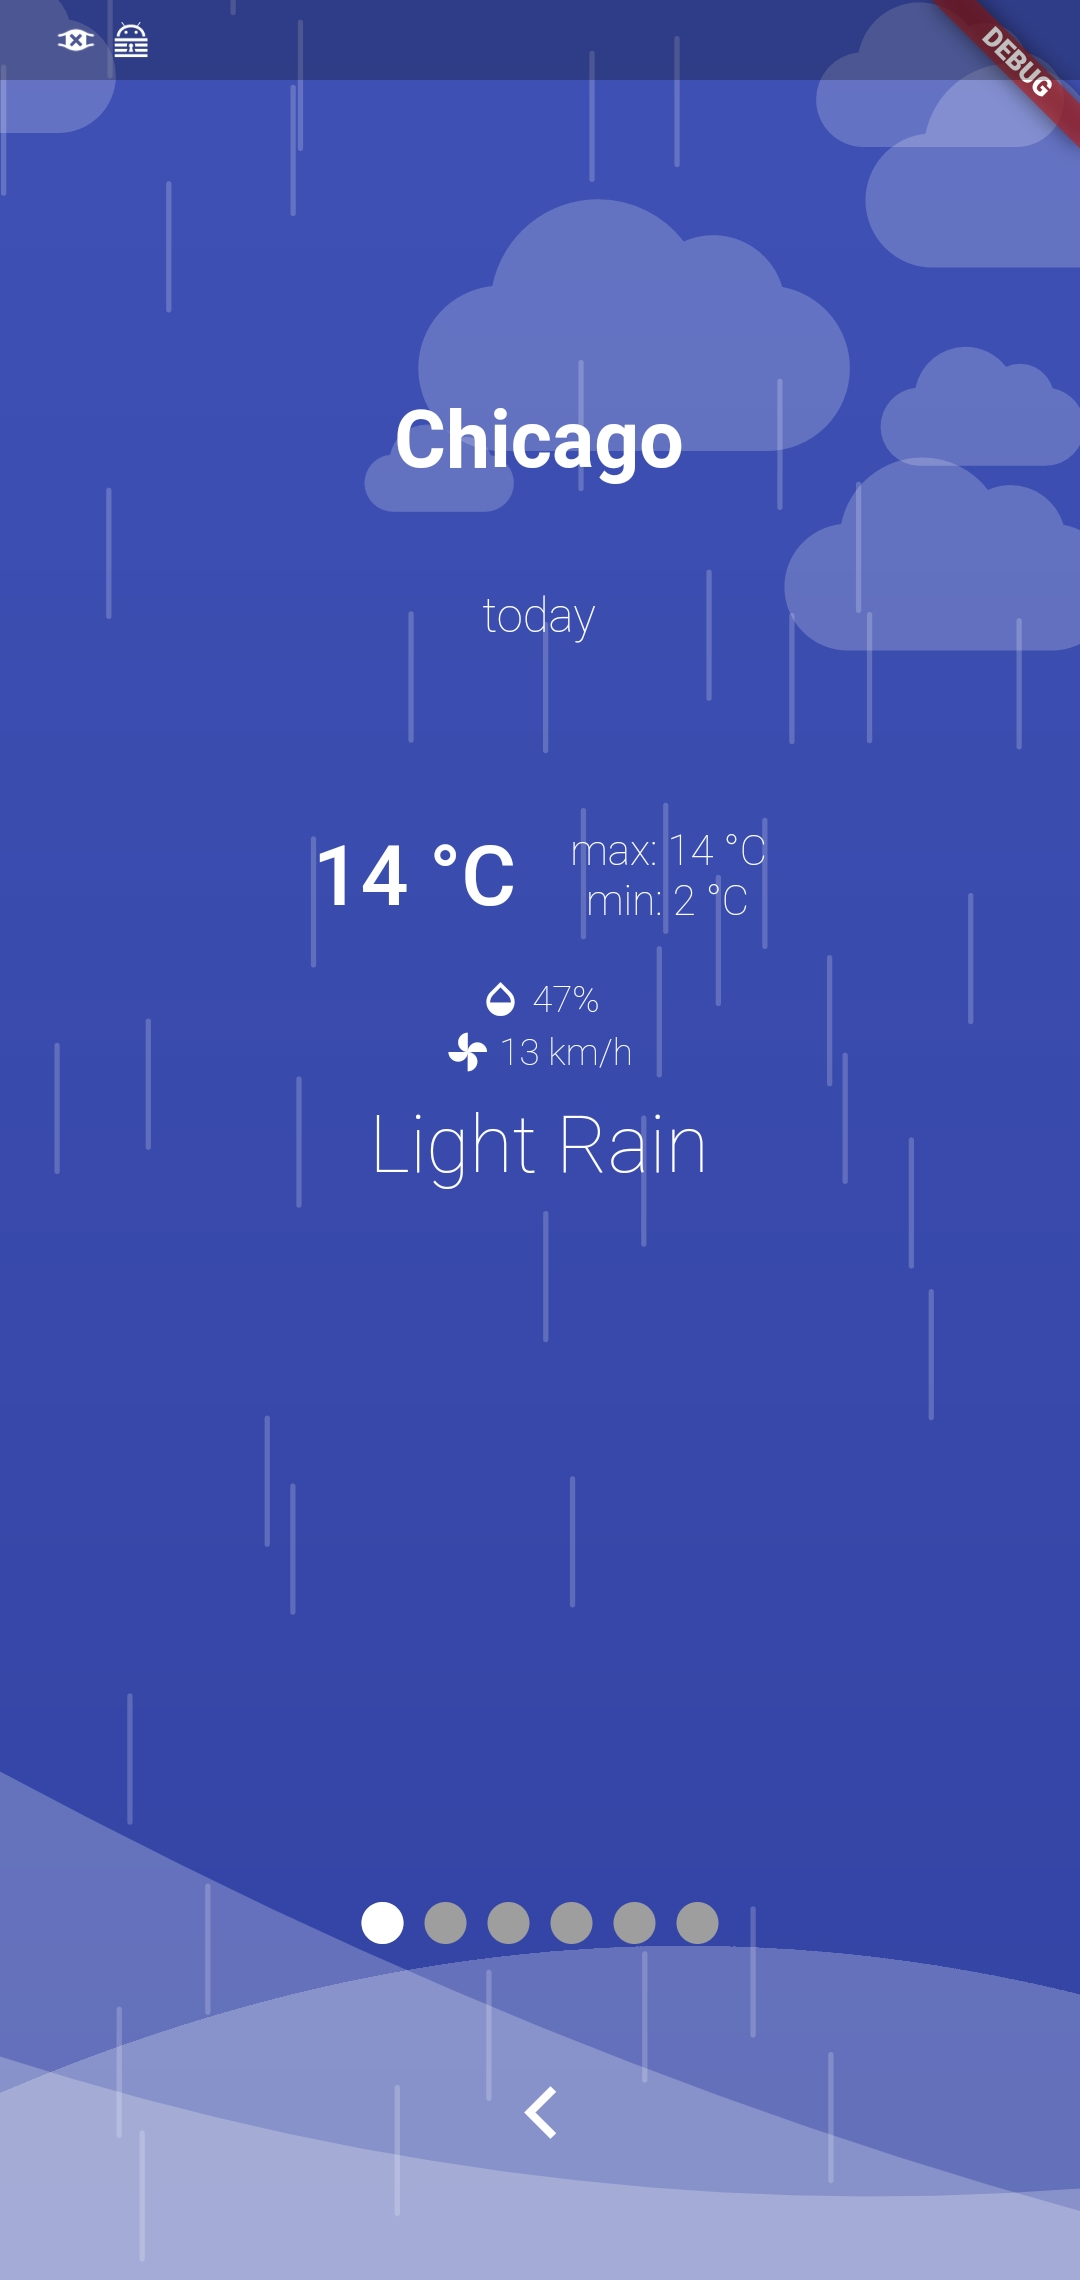
\includegraphics[width=\linewidth]{img/app-rain.jpg}
\endminipage\hfill
\minipage{0.32\textwidth}
  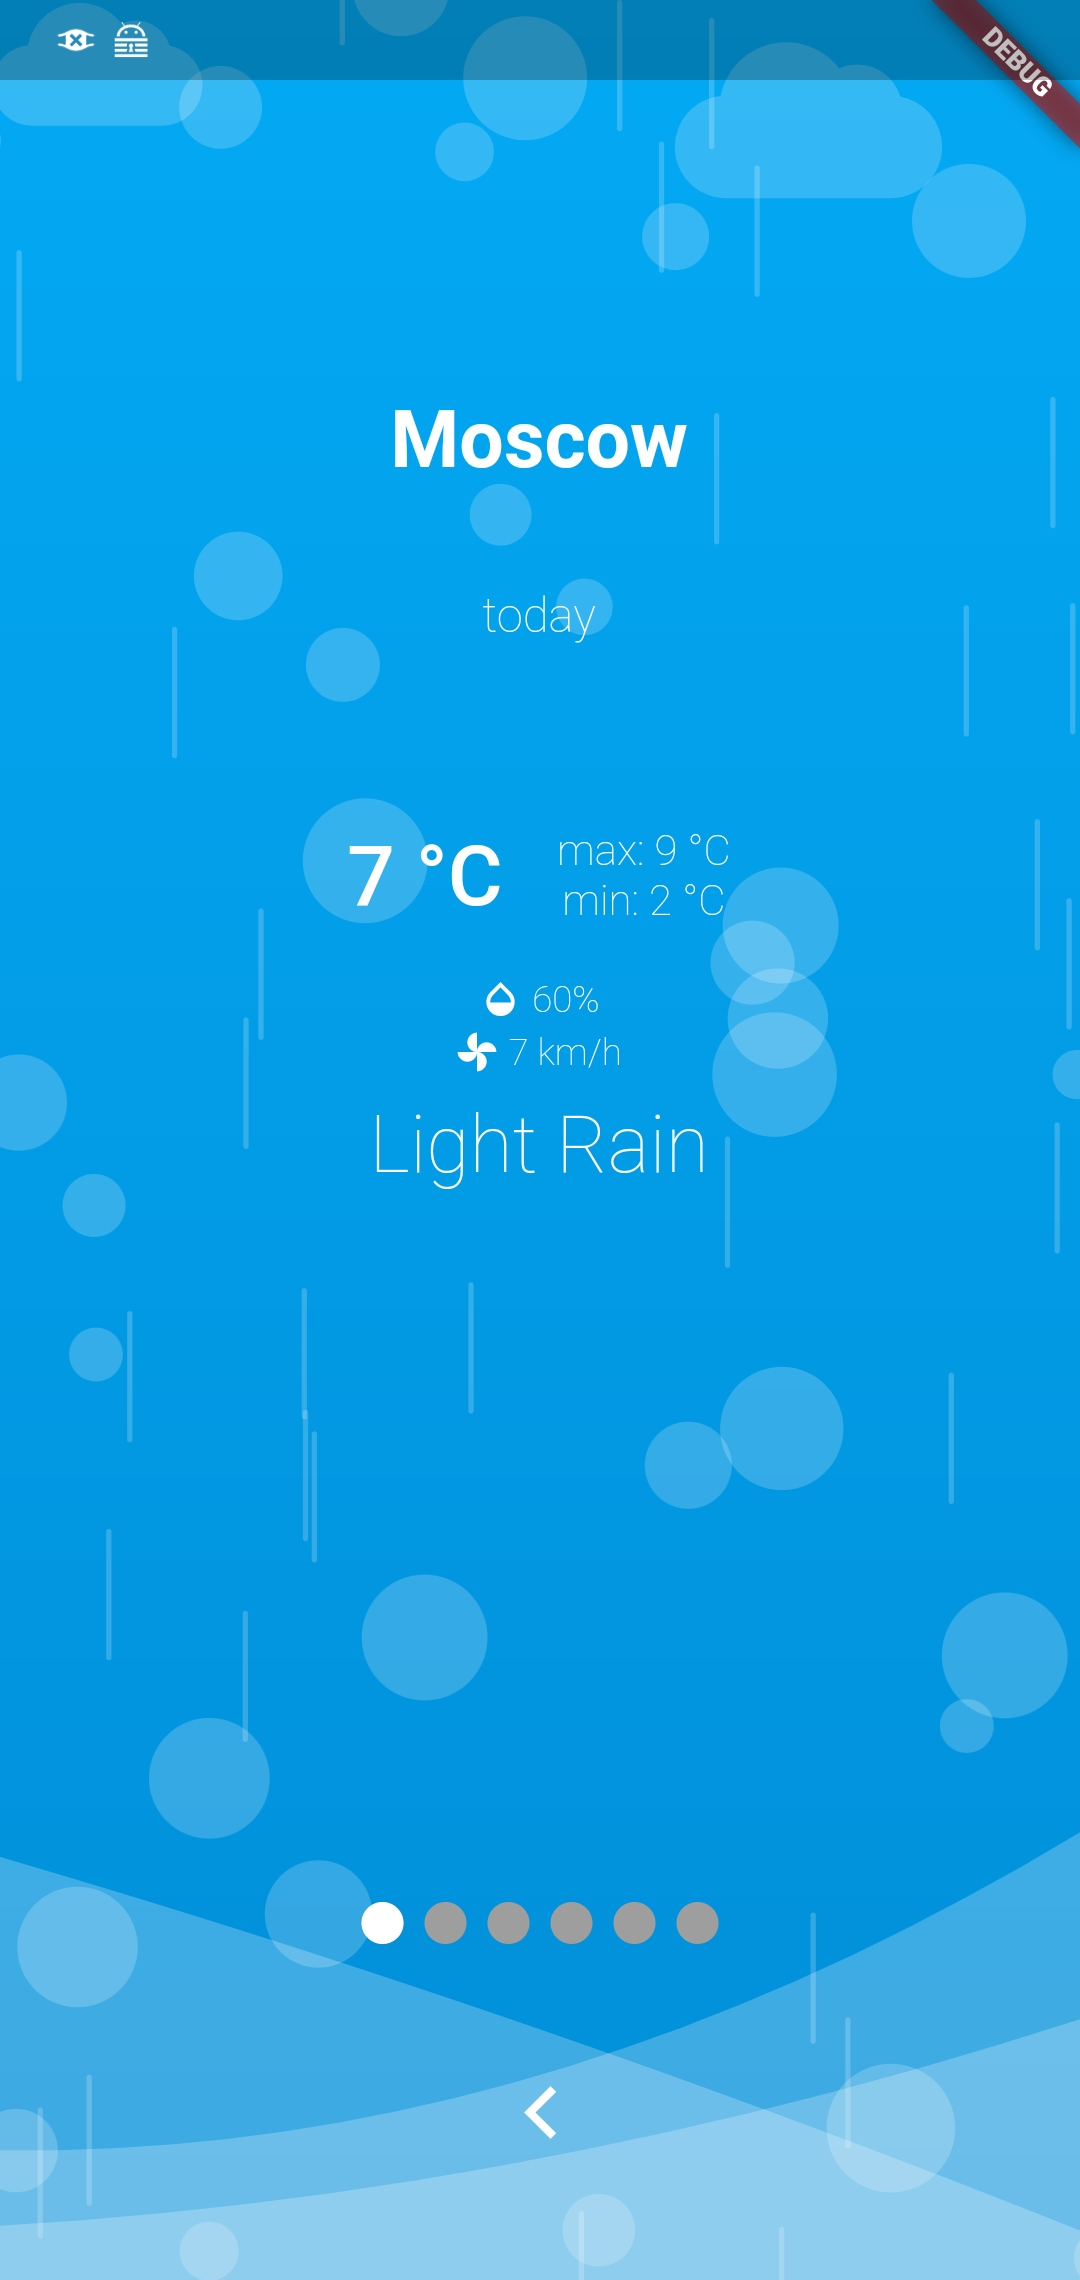
\includegraphics[width=\linewidth]{img/app-sleet.jpg}
\endminipage\hfill
\minipage{0.32\textwidth}%
  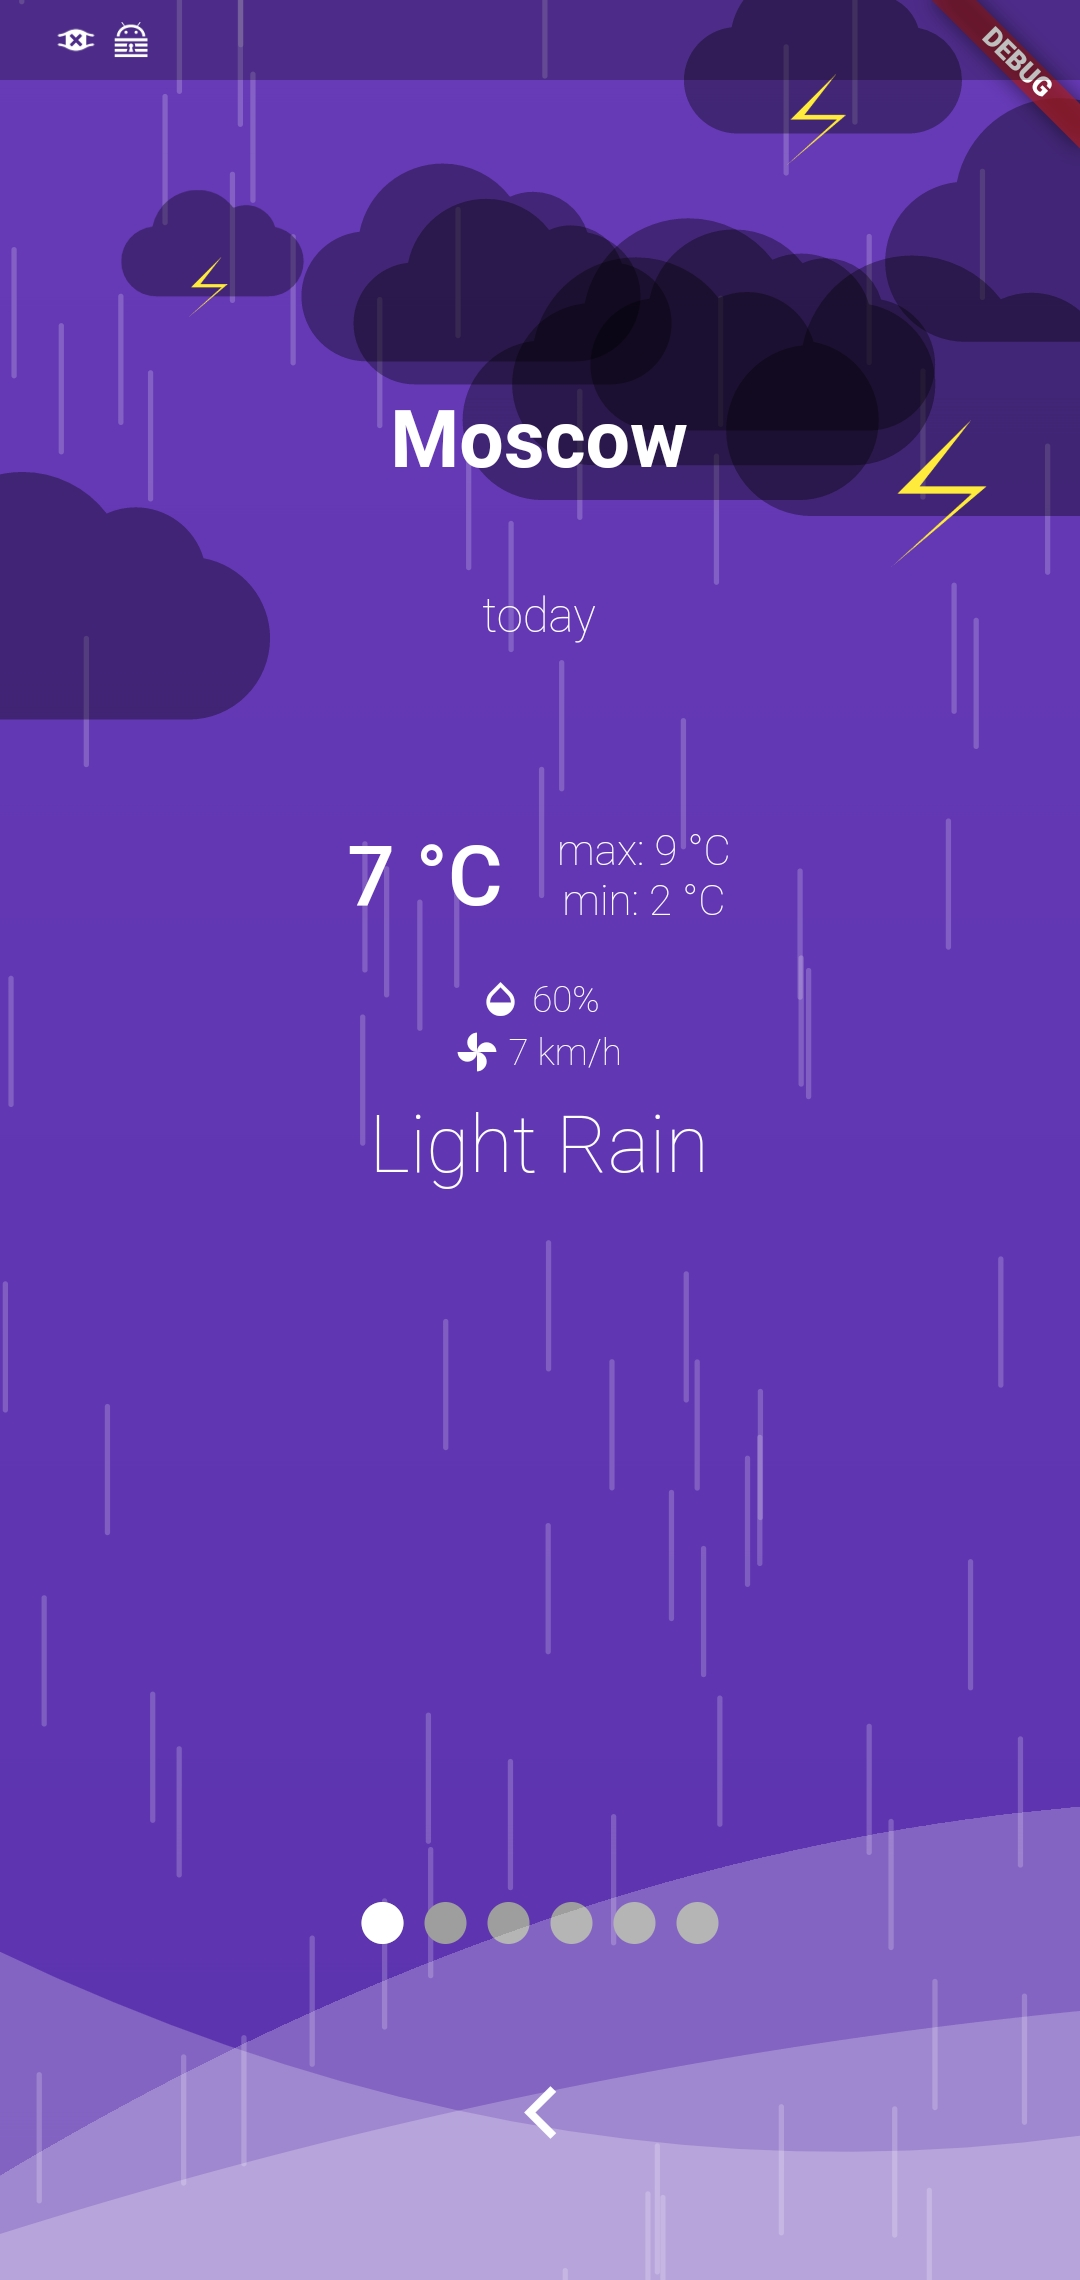
\includegraphics[width=\linewidth]{img/app-thunder.jpg}
\endminipage

  \caption{Ukázka různých typů počasí, jež aplikace vizualizuje}\label{fig:awesome_image1}
\end{figure}

\subsection{Dialog s nastavením aplikace}

V tomto dialogu, jež se otevře po kliknutí na ikonu ozubeného kola umístěného na v levém horním rohu úvodní obrazovky, má uživatel možnost pomocí přepínače přepnout nastavení, jestli se mají v aplikaci používat metrické nebo imperiální jednotky. Tato preference je uložena napříč jednotlivými spuštěními aplikace.

Pod přepínačem metrických a imperiálních jednotek se nachází tlačítko, jež slouží pro vymazání historie jich vyhledaných měst.

\begin{figure}[!ht]
\centering
{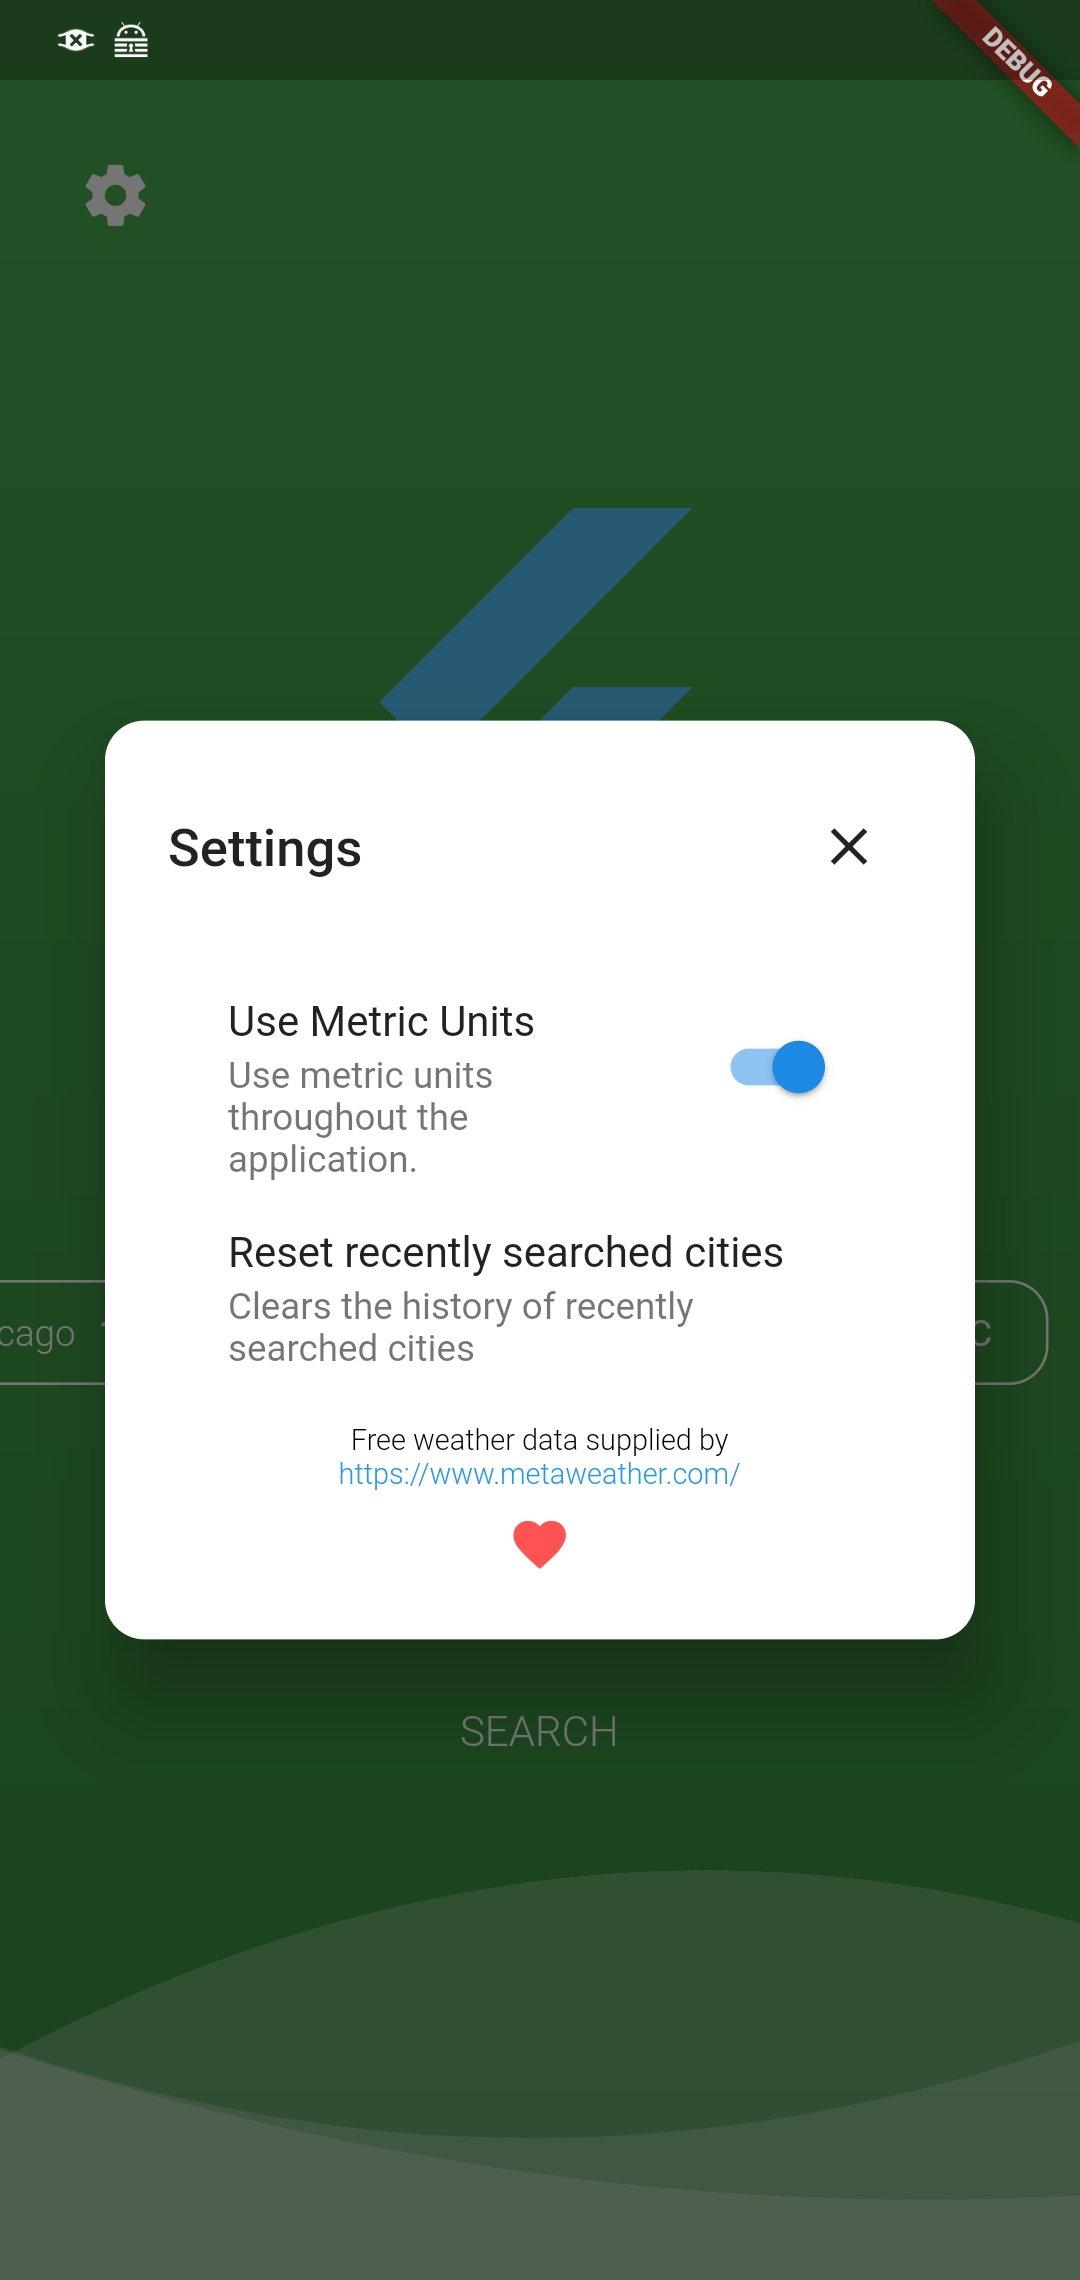
\includegraphics[width=0.40\textwidth]{img/app-settings.jpg}}
\caption{Dialog s nastavením aplikace}
\label{fig:flutter-architecture}
\end{figure}

Kliknutím na odkaz použité služby pro získávání předpovědi počasí je ve výchozím internetovém prohlížeči zařízení otevřena domovská stránka této služby.

\section{Popis implemtance}


\subsection{Správa stavů aplikace}

Při vývoji mobilních aplikací ve frameworku Flutter se často setkáváme s~pojmem \textbf{state management}, jež lze volně přeložit do češtiny jako \textbf{správa stavů aplikace}. Tento pojem se při využití tohoto frameworku používá proto, že narozdíl od vývoje nativních aplikací se pro tvorbu uživatelského rozhraní v~knihovně Flutter využívá spíše deklarativního paradigmatu, kdy se jasně deklarují jednotlivé stavy, ve kterých se aplikace může nacházet. Základní myšlenku tvorby uživatelského rozhraní v~tomto frameworku představuje následující rovnost:

\begin{figure}[!ht]
\center
$
uživatelské\_rozhraní = f(stav\_aplikace)
$
\end{figure}

V~praxi to znamená, že v~celém kódu Flutter aplikace například nelze nalézt žádné imperativní volání nastavení textu komponenty pro zobrazení textu na obrazovce, kdy se například na platformě Android v~nativním vývoji pro tuto operaci používá metoda \texttt{setText}. Každá část aplikace může mít vlastní stav, který se v~kódu implementuje tak, že se vytvoří potomek třídy \texttt{State} a~nadefinují se jednotlivé atributy tohoto stavu. Při aktualizaci stavu se tato celá část aplikace vykreslí znovu. Tento koncept lze nejlépe pochopit na následující ukázce kódu:

\begin{lstlisting}[language=Java,caption={Jednoduchá demonstrace aktualizace uživatelského rozhraní ve frameworku Flutter},captionpos=b, label={lst:sm-showcase}]
class _MyHomePageState extends State<MyHomePage> {
  int _counter = 0;
  void _incrementCounter() {
    // setState method forces the UI to redraw by
    // saying the state of the screen has changed
    setState(() {
      _counter++;
    });
  }

  @override
  Widget build(context) {
    return Scaffold(
      body: Center(
        child: Text(
          'Counter value: ' + _counter.toString(),
        ),
      ),
      floatingActionButton: FloatingActionButton(
          onPressed: _incrementCounter),
    );
  }
}
\end{lstlisting}

Avšak při vývoji složitejší aplikace brzy zjistíme, že při definici velké množiny stavů se bez sofistikovanější správy stavů kód aplikace brzy stane nepřehledným. Přístup ukázaný v~ukázce \ref{lst:sm-showcase} slouží jen k~demonstraci konceptu aktualizace uživatelského rozhraní a~nepředstavuje vhodné řešení manažementu stavů aplikace. V~praxi se zásadně používají komunitou vytvořené knihovny, mezi které například patří \texttt{provider}, \texttt{MobX}, \texttt{redux} nebo \texttt{flutter\_bloc}. Jelikož aplikace pro rozpoznávání registračních značek vozidel je netriviální aplikací, tak pro správu stavů složitejších obrazovek a~komponent byla zvolena knihovna \texttt{flutter\_bloc}, jež implementuje architekturu \textbf{BloC}.

\subsection{Použitá architektura pro správu stavů}

Ve vytvořené aplikaci je pro správu stavů použita architektura BloC (Bussiness Logic Components), jež rozděluje kód aplikací do tří hlavních částí:
\begin{itemize}
        \item \textbf{data} - datová část je zodpovědná za uložení a~manipulaci s~daty aplikace
        \item \textbf{byznysová logika} - úkolem této vrstvy je reagovat na události z~prezentační vrstvy novými stavy aplikace
        \item \textbf{prezentační vrsva} - uživatelské rozhrání aplikace je vykreslováno na základě získaného stavu z~byznysové logiky
\end{itemize}

\begin{figure}[!ht]
\centering
{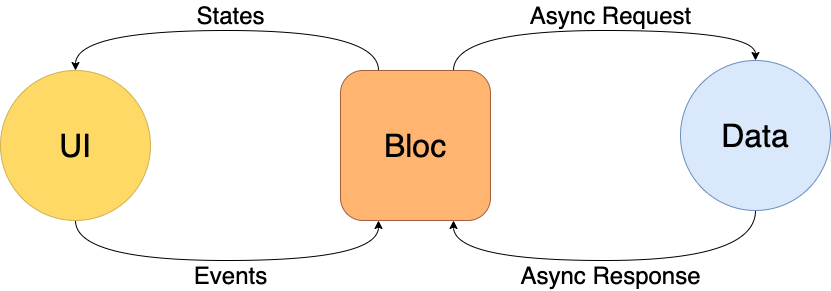
\includegraphics[width=13.5cm]{img/bloc-architecture.png}}
\caption{Diagram architektury BloC}
\label{fig:vrp-recognition-diagram}
\end{figure}

Obsluha jednotlivých událostí je asynchronní a~prezentační vrstvě může být během jedné obsluhy události předáno několik stavů.


\subsection{Manažement stavů procesu získávání předpovědi počasí}

Pro manažement stavů procesu získávání předpovědi počasí je vytvořena komponenta byznysové logiky \texttt{WeatherBloc}, jež reaguje na následující události:

\begin{itemize}
	\item \textbf{FetchWeather} - událost, která je vyvolána při vyhledání předpovědi počasí dle názvu města. Obsluha této události se nejdříve dotázá MetaWeather API na ID lokace dle názvu města. Pokud je dle názvu města nalezena nějaká lokace, tak tato obsluha dále již konkrétní předpověď pro nalezenou lokaci. Před vyhledáním předpovědi je vrácen stav \texttt{WeatherLoading}. Po úspěšném získání předpovědi je vrácen stav \texttt{WeatherLoaded}. V případě neúspěchu získávání je vrácen stav \texttt{WeatherError}
	\item \textbf{FetchWeatherByLocationId} - obsluha této události je velmi podobná obsluze události \texttt{FetchWeather} s tím rozdílem, že již je známé ID lokace ke které chceme získat předpověď, tudíž můžeme pomocí API vyhledat rovnou předpověď pro danou lokaci. Tato událost je vyvolávána položkami v historii již vyhledaných lokací.

		

\section{Závěr}
    V rámci této semestrální práce byl vytvořena dvojice programů - server a klient napodující deskovou hru Kris Kros. Důkladný a pečlivý návrh protokolu se osvědčil a v průběhu vývoje neprošel žádnými změnami. Avšak co se několikrát měnilo, byl způsob čtení zpráv, kdy nakonec jsou zprávy čteny spolehlivým automatem. Pokud bych automat navrhl hned na začátku, mohl jsem si ušetřit spoustu času laděním a upravováním parseru zpráv. Aplikace i server jsou však nyní funkční a hra je hratelná. Pokud je spojení s některým hráčem dočasně nedostupné nebo je klient násilně vypnut, tak po autorizaci je hráčovo stav korektně obnoven.
    


%obrazek
%\begin{figure}[!ht]
%\centering
%{\includegraphics[width=12cm]{img/poly-example.jpeg}}
%\caption{Zjednodušené UML aplikace (pouze balíčky)}
%\label{fig:photo}
%\end{figure}

	
	

\end{document}    
